\documentclass{article}
\usepackage{waspaa23}
\usepackage[dvipdfmx]{graphicx}
\usepackage{xcolor}
\usepackage{amsmath}
\usepackage{amsfonts}
\usepackage{url}

\usepackage{cite}
% \usepackage{times}
\usepackage[nolist,nohyperlinks]{acronym}
\usepackage{flushend}

\usepackage{bm}
\usepackage{booktabs}
\usepackage{siunitx}
\usepackage{subcaption}
\usepackage{cleveref}

\usepackage{bsssym}

\title{Rotation Robust Online Independent Vector Analysis with\\Sound Field Interpolation of Circular Microphone Array}
\name{%
  Taishi Nakashima \textsuperscript{\textdagger},
  Yukoh Wakabayashi \textsuperscript{\textdaggerdbl},
  Nobutaka Ono \textsuperscript{\textdagger}
  \thanks{This work was supported by JST CREST Grant Number \mbox{JPMJCR19A3} and JSPS KAKENHI Grant Number \mbox{JP21J22039}, Japan.}
}
\address{%
  \begin{minipage}{.5\textwidth}
    \begin{tabular}{@{}c@{}}
      \textsuperscript{\textdagger}
      Graduate School of Systems Design,\\
      Tokyo Metropolitan University\\
      {\small 6--6, Asahigaoka, Hino-shi, Tokyo 191--0065, Japan}\\
      {\footnotesize \url{nakashima-taishi@ed.tmu.ac.jp}, \url{onono@tmu.ac.jp}}
    \end{tabular}
  \end{minipage}
  \hfill
  \begin{minipage}{.5\textwidth}
    \begin{tabular}{@{}c@{}}
      \textsuperscript{\textdaggerdbl}
      Graduate School of Engineering,\\
      Toyohashi University of Technology\\
      {\small 1--1 Hibarigaoka, Tempaku-cho, Toyohashi, Aichi, 441--8580}\\
      {\footnotesize \url{wakayuko@cs.tut.ac.jp}}
    \end{tabular}
  \end{minipage}
}

% % for DeepL
% \rhead{}
% \chead{}
% \lhead{}

\begin{document}
\maketitle
% \onecolumn

\begin{abstract}
  % 本論文では,マイクロホンアレイの回転に頑健なオンラインブラインド音源分離手法を提案する.
  % Online auxiliary-function-based independent vector analysis (OIVA)はリアルタイムBSSを実現するための有望な手法のひとつである.
  % リアルタイムBSSを実用化するためには,音源やマイクの移動といった環境の変化に対する頑健性が重要な課題である.
  % OIVAでは音源のなめらかな移動に対して頑健かつ高い分離性能を獲得できることが示されていた.
  % しかし,OIVAはマイクの突発的な移動に対しては十分な性能が得られない.
  % そこで本論文では,円状等間隔マイクロホンアレイ(CMA)に対する音場補間処理をOIVAの前処理として活用することを試みる.
  % シミュレーション実験により音場補間によって音源分離性能が向上したことを確認した.
  In this paper, we propose an online blind source separation (BSS) method that is robust against rotation of microphone arrays.
  Online auxiliary-function-based independent vector analysis (OIVA) is one of the promising methods for real-time BSS.
  A key issue for practical real-time BSS is robustness against environmental changes such as source and microphone movement.
  OIVA has been shown to be robust against smooth movement of sources and to achieve high separation performance.
  However, OIVA does not perform well against sudden movements of microphones.
  Therefore, in this paper, we attempt to employ the sound field interpolation for circular microphone arrays (CMAs) as a pre-processing for OIVA.
  Simulation experiments confirmed that the sound field interpolation improves the source separation performance.
\end{abstract}
\begin{keywords}
  Blind source separation,
  online source separation,
  independent vector analysis,
  circular microphone array,
  sound field interpolation
\end{keywords}

\section{Introduction}
% ブラインド音源分離など多くのアレイ信号処理では,時不変な系を仮定する.
% しかし,実応用のためにはマイクロホンや音源の移動など系の時間変化を考慮する必要がある.
% そこで,系の時間変化のひとつとして,円状等間隔マイクロホンアレイ(circular microphone array; CMA)の回転を考え,音場の補間により対応する手法 \cite{Wakabayashi:2020:ASJ:A} が提案された.
% この手法はCMAの対称性を利用することで,CMAが回転する前の音場を簡単な線形演算により推定する.
% また,ビームフォーミング \cite{Wakabayashi:2021:ICASSP} やステアリングベクトル推定 \cite{Wakabayashi:2021:ASJ:A} への応用や,
% CMAの回転角度を自己推定する手法 \cite{Lian:2021:APSIPA} も提案されている.
% 本稿では,CMAが回転する状況下のブラインド音源分離に取り組む.
% 音場補間によりCMAの回転の影響を打ち消し,後段にブラインド音源分離を適用する.
% さらに,シミュレーション実験により音源分離性能を評価する.
Most array signal processing methods, such as blind source separation (BSS), assume a time-invariant system.
However, for practical applications, it is necessary to consider time variations of the system, such as movements of the microphone or source.
Sound field interpolation for circular microphone array (CMA) \cite{Wakabayashi:2021:ICASSP} has been proposed to address the rotation of a CMA as one of the time variations of the system.
This method exploits the symmetry of the CMA to estimate the sound field before the rotation of the CMA by a simple linear operation.
Applications to beamforming \cite{Wakabayashi:2021:ICASSP} and steering vector estimation \cite{Wakabayashi:2021:ASJ:A} have also been proposed,
as well as a method for self-estimating the rotation angle of a CMA \cite{Lian:2021:APSIPA}.
In this paper, we address blind source separation in situations where the CMA rotates.
The effect of the rotational movement of the CMA is counteracted by interpolating the sound field, and blind source separation is applied in the latter stage.
Furthermore, the source separation performance is evaluated by simulation experiments.

\section{Formulation}
% 音源の数を$\Src$,マイクの数を$\Mic$とする.
% 短時間フーリエ変換領域において,観測信号$\obs _{\ft} \in \C ^{\Mic}$は
% \begin{equation}
%   \obs _{\ft} = \sum _{\src=1} ^{\Src} \steer _{\src\ft} \sig _{\src\ft},
% \end{equation}
% でモデル化されると仮定する.
% ただし,
% $\freq = 1, \dots, \Freq$は周波数ビンインデクス,
% $\tframe = 1, \dots, \Tframe$は時間フレームインデクス,
% $\sig _{\src\ft} \in \C\; (\src = 1, \dots, \Src)$は$\src$個目の音源信号,
% $\steer _{\src\ft} \in \C ^{\Mic}\; (\src = 1, \dots, \Mic)$はそのステアリングベクトルである.
Let $\Src$ and $\Mic$ respectively be the number of sources and microphones.
We assume that the observed signal $\obs _{\ft}$ is modelled as:
\begin{equation}
  \obs _{\ft} = \sum _{\src=1} ^{\Src} \steer _{\src\ft} \sig _{\src\ft},
\end{equation}
in the short-time Fourier transform (STFT) domain,
where $\freq = 1, \dots, \Freq$ denotes the frequency bin index,
$\tframe = 1, \dots, \Tframe$ denotes the time frame index,
$\sig _{\src\ft} \in \C\; (\src = 1, \dots, \Src)$ denotes the $\src$-th source signal, and
$\steer _{\src\ft} \in \C ^{\Mic}\; (\src = 1, \dots, \Mic)$ denotes the steering vector of $\src$th source signal to each microphone.

% オンラインブラインド音源分離の目的は,現在と過去の観測信号$\{\obs _{\freq,i}\} _{i=1} ^{\tframe}$のみを用いて,
% 分離行列を推定し,音源を分離することである:
% \begin{align}
%   \Demix _{\ft} &= \begin{bmatrix} \demix _{1\ft} & \dots & \demix _{\Src\ft} \end{bmatrix} ^{\hermite} \in \C ^{\Src \times \Mic}, \\
%   \est _{\ft} &= \Demix _{\ft} \obs _{\ft} \in \C ^{\Src},
% \end{align}
% ここで,$\Demix _{\ft}$は分離行列,$\est _{\ft}$は分離信号である.
% 本研究では,ある時間フレーム$\rotFra$においてCMAが角度$\rotDeg$回転した状況下で分離行列を推定することを考える.
% ただし,$\rotFra$および$\rotDeg$は既知とする.
Online blind source separation aims to estimate the demixing matrix and estimated signals using only the current and past observed signals $\{\obs _{\freq,i}\} _{i=1} ^{\tframe}$:
\begin{align}
  \Demix _{\ft} &= \begin{bmatrix} \demix _{1\ft} & \dots & \demix _{\Src\ft} \end{bmatrix} ^{\hermite} \in \C ^{\Src \times \Mic}, \\
  \est _{\ft} &= \Demix _{\ft} \obs _{\ft} \in \C ^{\Src},
\end{align}
where $\Demix _{\ft}$ is the demixing matrix and $\est _{\ft}$ is the estimated signal.
We consider estimating the demixing matrix in a situation where the CMA is rotated by an angle $\rotDeg$ in a certain time frame $\rotFra$.
In this study, $\rotFra$ and $\rotDeg$ are assumed to be known.

\section{Proposed method}
{%
  \color{red}\bf
  式迷走中… $\rotObs _{\ft}$は回転後の観測信号とするか,回転を補償した後の観測信号とするかで$\rotMat$のかけ方が変わる.
  若林先生のASLP論文では$\rotObs _{\ft} = \rotMat (-\rotDeg) \obs _{\ft}$と書いていて,$\obs _{\ft}$は回転後の信号としている?
}

音場補間は,CMAが回転した後の位置における観測信号$\rotObs _{\ft}\; (\tframe \geq \rotFra)$のみを用いて,
CMAの回転をキャンセルする行列$\rotMat (\rotDeg) \in \C ^{\Mic\times\Mic}$を推定することを目指す:
\begin{equation}
  \obs _{\ft} = \rotMat (\rotDeg) \rotObs _{\ft},
\end{equation}
$\rotMat (\rotDeg)$の計算方法の詳細は文献 \cite{Wakabayashi:2020:ASJ:A} を見よ.
$\rotMat (\rotDeg)$が推定できれば,CMAが回転する前の位置における観測信号は$\obs _{\ft} = $
CMAが回転する前の時間フレーム$\tframe < \rotFra$における観測信号$\obs _{\ft}$を用いて分離行列$\Demix _{\ft}$が推定できていたとする.
音場補間を適用し,回転前の観測信号を推定することで,CMAが回転した後も分離行列を推定し直すことなく分離信号$\est _{\ft}$が得られる.
\begin{equation}
  \est _{\ft} = \Demix _{\ft} \rotObs _{\ft} = \Demix _{\ft} \left(\rotMat (\rotDeg)^{-1} \obs _{\ft}\right).
\end{equation}

本論文では,補助関数型独立ベクトル分析 (auxiliary-function-based independent vector analysis; AuxIVA) \cite{Ono:2011:WASPAA}
およびそのオンライン拡張 (online AuxIVA; OIVA) \cite{Taniguchi:2014:HSCMA} を用いて音源分離を行う.
AuxIVAでは,各音源$\src = 1, \dots, \Src$に対して次の更新式で時不変な分離行列$\Demix _{\freq}$を推定する.
\begin{align}
  \srcvar _{\src\tframe} &\gets \sqrt{\sum _{\freq=1} ^{\Freq} \lvert \demix ^{\hermite} _{\src\freq} \obs ^{\nohermite}_{\ft} \rvert ^2}, \\
  \cov _{\src\freq} &\gets \frac{1}{\Tframe} \sum _{\tframe=1} ^{\Tframe} \weight (\srcvar_{\src\tframe}) \obs _{\ft} \obs _{\ft}^{\hermite}, \\
  \demix _{\src\freq} &\gets (\Demix _{\freq} \cov _{\src\freq}) ^{-1} \bm{e} _{\src} \label{eq:ip:proj}, \\
  \demix _{\src\freq} &\gets {\demix _{\src\freq}} / {\sqrt{\demix _{\src\freq} ^{\hermite} \cov _{\src\freq} \demix _{\src\freq}}} \label{eq:ip:norm}.
\end{align}
ここで,$\bm{e}_{\src}$は単位行列の$\src$列目のベクトルである.
$\cov _{\src\freq}$は{重み付き共分散行列}と呼ばれる.
$\weight(\srcvar)$は音源モデルによって定まる関数であり,
本論文では時変Gauss分布$\weight (\srcvar) = \Freq/{\srcvar ^2}$ \cite{Ono:2012:APSIPA}を用いる.

一方OIVAでは,各時間フレーム$\tframe$ごと重み付き共分散行列$\cov _{\src\ft}$を更新する~\cite{Taniguchi:2014:HSCMA}.
\begin{equation}
  \cov _{\src\ft} \gets \forget \cov _{\src\freq(\tframe-1)} + (1 - \forget) \weight ({\srcvar _{\src\tframe}}) \obs _{\ft} \obs _{\ft}^{\hermite}.
\end{equation}
ここで,$\forget\; (0 \leq \forget < 1)$は忘却係数である.
分離行列は\cref{eq:ip:proj}, \cref{eq:ip:norm}と同じ更新式を用いて書く時間フレームで更新する.
両方の手法において,CMAの回転を含む観測信号に対して,音場補間を適用した後の信号を改めて入力する.

% It is shown how to approximate x̂=U(θ)x using a certain matrix U (θ) ∈ CM ×M, with the observed signal x̂ (t ≥ t̂) at the position after the microphone has rotated (see [1] for details).
% Suppose that the separation matrix W could be estimated using the observed signal x in time frame t<t̂ before the CMA was rotated.
% By applying sound field interpolation and estimating the observed signal before the rotation as follows, the separation signal y can be obtained after the CMA has rotated without having to re-estimate the separation matrix.

% In this paper, auxiliary-function-based independent vector analysis (AuxIVA) [5] and its online extension (online AuxIVA; OIVA) [6] are used as source separation methods.
% In AuxIVA, each source k = 1, . . . K, the time-invariant separation matrix W is estimated with the following update formula

% where ek is the kth column vector of the identity matrix.
% Vkf is called the weighted covariance matrix.
% φ(r) is a function determined by the source model, and in this paper the time-invariant Gauss distribution φ(r) = F/r2 [7].
% OIVA, on the other hand, updates the weighted covariance matrix Vkf t for each time frame t [6].
% where α (0 ≤ α < 1) is the forgetting factor. The separation matrix is updated in the time frame in which it is written using the same update formula as in eq. (8), eq. (9).
% For both methods, the signal is input again after applying the sound field interpolation to the observed signal including the CMA rotation.

\subsection{Frequency band limitation}
TBD
\begin{itemize}
  \item 音場補間は周波数が高くなるほどモデルとの乖離が大きくなり補間性能が悪くなる \cite{Wakabayashi:2020:ASJ:A}
  \item 音源分離に用いる音源モデル$\srcvar _{\src\tframe}$を計算するとき,補間がうまくできている周波数帯域だけで計算すれば分離性能が改善されると期待できる
  \item サンプリング周波数$\freqSamp~\unit{\hertz}$,FFT点数$\nfft$のとき,STFTの周波数ビンインデクス$\freq$と物理的な周波数$\freqPhys$の対応
    \begin{equation}
      \freqPhys = \frac{(\freq - 1)\times\freqSamp}{\nfft} \quad \left(\freq = 1, \dots, \frac{\nfft}{2} + 1\right),
    \end{equation}
  \item 修正された音源モデルの更新式
    \begin{equation}
      \srcvar _{\src\tframe} = \sqrt{\sum _{\freq = 1} ^{\SubFreq} \lvert \demix _{\src\ft} \obs _{\ft} \rvert ^2},
    \end{equation}
    ただし,$\SubFreq$は周波数の上限
\end{itemize}

\section{Simulated experiments}
\subsection{Setup}
% CMAが回転する条件下で,ブラインド音源分離の性能を評価した.
% 音源信号は,SiSECデータベース \cite{Araki:2012:LVAICA}から男性と女性の各1サンプル音源を用いた.
% 音源信号のサンプリング周波数は\SI{16}{\kilo\hertz}であり,長さ\SI{40}{\second}になるよう加工した.
% これらの信号を用いて鏡像法 \cite{Allen:1979:JASA} によるシミュレーションを行い音像を生成した.
% \Cref{fig:room}に鏡像法のためのマイクと音源の配置を示す.
% 残響時間は約\SI{100}{\milli\second}である.
% \begin{figure}[t]
%   \centering
%   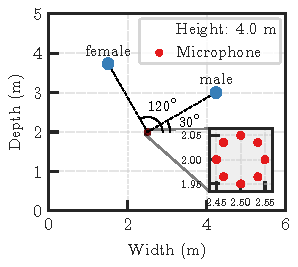
\includegraphics{figures/room_layout.pdf}
%   \caption{Room layout.}
%   \label{fig:room}
% \end{figure}
% マイクロホンアレイはマイク数$\Mic = 8$,半径\SI{5}{\cm}のCMAを用いた.
% CMAを\cref{fig:room}中の水平軸から反時計周りに0度,30度,45度回転させた場合の音像を生成し,
% それぞれ0--10\si{\second},10--25\si{\second},25--40\si{\second}の区間でつなぎ合わせることでマイクロホンアレイの回転を擬似的にシミュレートした.
% 得られた観測信号に対してフレーム長4096点,シフト長1024点,Hamming窓で短時間フーリエ変換を行い音源分離および音場補間を行った.
% AuxIVAおよびOIVAの分離行列の初期値は単位行列とした.
% 反復回数はAuxIVAは100,OIVAは2とした.
% OIVAは忘却係数$\forget$を\num{0.97},\num{0.99}および\num{0.995}と変化させて音源分離を行った.
% 音場補間を用いた観測信号と用いない観測信号それぞれについて音源分離を行い,scale-invariant signal-to-distortion ratio (SI-SDR) \cite{LeRoux:2019:ICASSP} とその改善量(以下,SDRi)をチャネルごとに平均した.
% 本実験では音場補間によってCMAの回転を補償した信号に対して音源分離を行うために,SI-SDRとSDRiの計算に用いる参照信号はCMAが回転していない場合の音像を用いた.
% また,OIVAにおいては,分離信号を\SI{1}{\second}ごとの区間に分割し,各区間でSDRiを計算した.

We evaluate the performance of OIVA under a condition where CMA rotated.
One male and one female source sample each from the SiSEC database \cite{Araki:2012:LVAICA} were used as the source signals.
The sampling frequency of the source signals was \SI{16}{\kilo\hertz} and they were processed to a length of \SI{40}{\second}.
These signals were used to generate a source image by simulation using the image source method \cite{Allen:1979:JASA}.
\Cref{fig:room} shows the microphone and source layout for the image source method.
\begin{figure}[t]
  \centering
  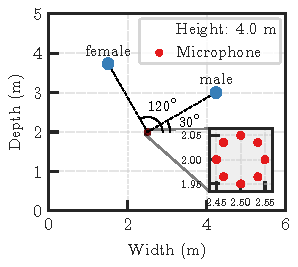
\includegraphics{figures/room_layout.pdf}
  \caption{Room layout.}
  \label{fig:room}
\end{figure}
The reverberation time is approximately \SI{100}{\milli\second}.
The microphone array consists of a CMA with $\Mic = 8$ microphones and a radius of \SI{5}{\centi\metre}.
The source images were generated when the CMA was rotated by 0°, 30° and 45° counterclockwise from the horizontal axis in \cref{fig:room},
and were stitched together in the intervals 0-10s, 10-25s and 25-40s, respectively, to simulate the rotation of the microphone array.
The rotation of the microphone array was simulated by joining the images at intervals of 0-10s, 10-25s and 25-40s, respectively.
%
STFT was applied to the observed mixture signals with a FFT length of 4096 points, a shift length of 1024 points and a Hamming window.
The initial values of the demixing matrices for AuxIVA and OIVA were unit matrices.
The number of iterations was set to 100 for AuxIVA and 2 for OIVA.
OIVA was performed by varying the forgetting factor $\forget$ from \num{0.97}, \num{0.99} and \num{0.995}.
The source separation was carried out on the observed signals with and without sound field interpolation,
and the scale-invariant signal-to-distortion ratio (SI-SDR) \cite{LeRoux:2019:ICASSP} and its improvement (SDRi) were averaged over the channels.
In this experiment, the reference signal used to calculate SI-SDR and SDRi was the source image when the CMA was not rotating, in order to perform source separation on the signal compensated for the rotational shift of the CMA by means of sound field interpolation.
For OIVA, the separated signal was divided into intervals of 1 s and SDRi was calculated for each interval.

\subsection{Results}
% まず,音場補間を用いない観測信号に対するAuxIVAの分離性能は\SI[round-mode=places,round-precision=3]{-5.104996}{\decibel}であり,十分な分離性能が得られなかった.
% これは,AuxIVAがバッチ処理であるためCMAの回転に追従できなかったためと考えられる.
% 次に,音場補間を用いた観測信号に対するAuxIVAの分離性能は\SI[round-mode=places,round-precision=3]{-1.094806}{\decibel}であった.
% 音場補間を用いない観測信号の結果と比較すると改善しているが,まだ十分な分離性能ではない.
% これは周波数が高くなるほど音場補間の性能が悪くなる現象によるものと考えられ,先行研究の結果と一貫している.
First, the separation performance of AuxIVA for the observed signal without sound field interpolation was -5.105 dB, which was insufficient.
This is considered to be because AuxIVA is a batch process and could not follow the rotation of the CMA.
The separation performance of AuxIVA for the observed signal with sound field interpolation was -1.095 dB.
This is an improvement compared to the results for the observed signal without sound field interpolation, but the separation performance is still not sufficient.
This is considered to be due to the phenomenon that the performance of the sound field interpolation worsens as the frequency increases, which is consistent with the results of previous studies.

% 次に,OIVAの結果を\cref{fig:online}に示す.
% \begin{figure}[t]
%   \centering
%   \begin{subfigure}[t]{\linewidth}
%     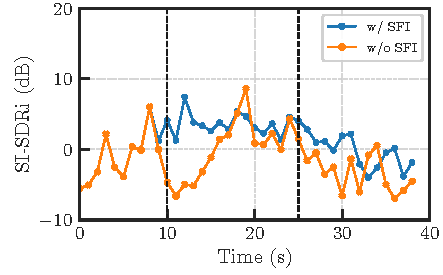
\includegraphics{figures/plots/online/Gauss_8000_97.pdf}
%     \caption{$\forget = 0.99$}
%   \end{subfigure}
%   \begin{subfigure}[t]{\linewidth}
%     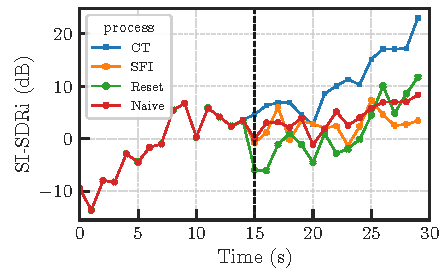
\includegraphics{figures/plots/online/Gauss_8000_99.pdf}
%     \caption{$\forget = 0.99$}
%   \end{subfigure}
%   \begin{subfigure}[t]{\linewidth}
%     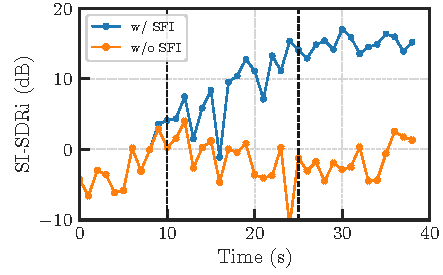
\includegraphics{figures/plots/online/Gauss_8000_995.pdf}
%     \caption{$\forget = 0.995$}
%   \end{subfigure}
%   \caption{Frame-wise SI-SDR improvements (dB). Two vertical dotted lines at \SI{10}{\second} and \SI{25}{\second} denote the rotaion of microphone array.}
%   \label{fig:online}
% \end{figure}
% 図中の縦の点線はCMAの回転を表す.
% まず,忘却係数$\forget=0.97$のとき,音場補間を適用した信号は,\SI{10}{\second}から\SI{25}{\second}の区間でおよそ\SI{5}{\decibel}の分離性能が得られているが,\SI{25}{\second}以降で分離性能が低下した.
% 忘却係数$\forget=0.99$のとき,前の結果と比較して全体的に分離性能が大きく改善しており,CMAの回転にも頑健であることが確認できる.
% 忘却係数$\forget=0.995$のとき,$\alpha = 0.99$の結果と比べて分離性能の増加が遅くなっているものの,CMAの回転後も\SI{10}{\decibel}付近の分離性能を維持できていることがわかる.

\begin{figure}[t]
  \centering
  \begin{subfigure}[t]{\linewidth}
    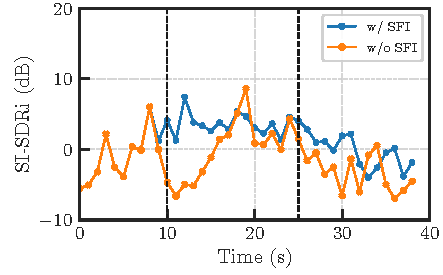
\includegraphics{figures/plots/online/Gauss_8000_97.pdf}
    \caption{$\forget = 0.99$}
  \end{subfigure}
  \begin{subfigure}[t]{\linewidth}
    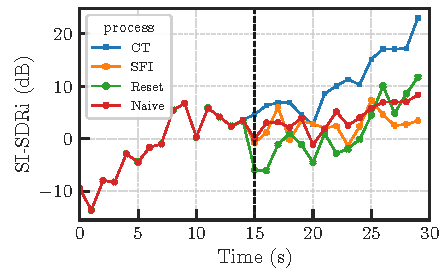
\includegraphics{figures/plots/online/Gauss_8000_99.pdf}
    \caption{$\forget = 0.99$}
  \end{subfigure}
  \begin{subfigure}[t]{\linewidth}
    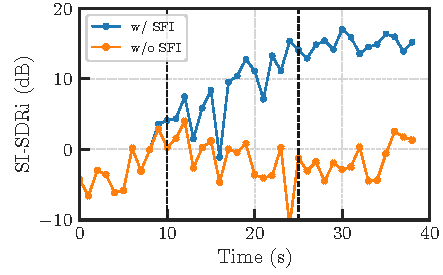
\includegraphics{figures/plots/online/Gauss_8000_995.pdf}
    \caption{$\forget = 0.995$}
  \end{subfigure}
  \caption{Frame-wise SI-SDR improvements (dB). Two vertical dotted lines at \SI{10}{\second} and \SI{25}{\second} denote the rotaion of microphone array.}
  \label{fig:online}
\end{figure}
Next, the OIVA results are shown in \cref{fig:online}.
The vertical dotted line in the figure represents the rotation of the CMA.
When the forgetting factor $\forget = 0.97$, the signal to which the sound field interpolation was applied showed a separation performance of approximately 5 dB in the interval from 10 s to 25 s.
However, the separation performance decreased after 25 s. The results are consistent with the results of previous studies.
When the forgetting factor $\forget = 0.99 $, the overall separation performance improves significantly compared to the previous results, confirming that it is robust to CMA rotation.
When the forgetting factor $\forget = 0.995$, the separation performance increases more slowly compared to the results with $\forget = 0.99$, but it can be seen that the separation performance remains around 10 dB after the rotation of the CMA.

\section{Conclusion}
% 本研究では,円状等間隔マイクロホンアレイにおける音場補間をブラインド音源分離に応用した.
% シミュレーション実験により,音場補間が円状等間隔マイクロホンアレイの回転に対するOIVAの頑健性を改善させたことを確認した.
% 今後は本手法の自己回転角度推定 \cite{Lian:2021:APSIPA} との組み合わせや,実時間処理への拡張などに取り組む.
In this study, sound field interpolation for an equally spaced circular microphone array (CMA) was applied to online auxiliary-function-based independent vector analysis (OIVA).
Simulation experiments have confirmed that sound field interpolation improved robustness of OIVA against the rotation of CMA.
Future work includes combining this method with self-rotation angle estimation \cite{Lian:2021:APSIPA} and extending it to real-time processing.

% \section*{Acknowledgments}
% This work was supported by JST CREST Grant Number \mbox{JPMJCR19A3} and JSPS KAKENHI Grant Number \mbox{JP21J22039}, Japan.
\clearpage\newpage
\bibliographystyle{IEEEtran}
\bibliography{IEEEabrv,ref}

\clearpage\newpage
\onecolumn
\section*{Results of frequency band limitation}
\newcommand{\myscale}{.75}
\begin{figure*}[h]
  \centering
  \begin{subfigure}[t]{.3\textwidth}
    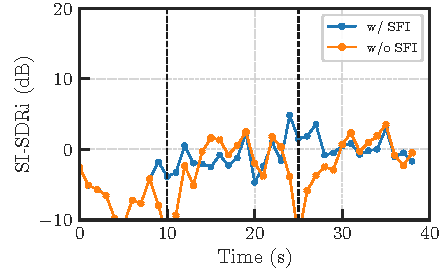
\includegraphics[scale=\myscale]{figures/plots/online/Gauss_2000_97.pdf}
    \caption{$\SubFreq = 2000$}
  \end{subfigure}
  \begin{subfigure}[t]{.3\textwidth}
    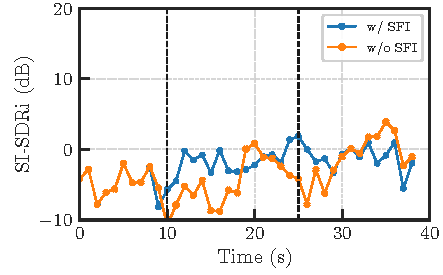
\includegraphics[scale=\myscale]{figures/plots/online/Gauss_4000_97.pdf}
    \caption{$\SubFreq = 4000$}
  \end{subfigure}
  \begin{subfigure}[t]{.3\textwidth}
    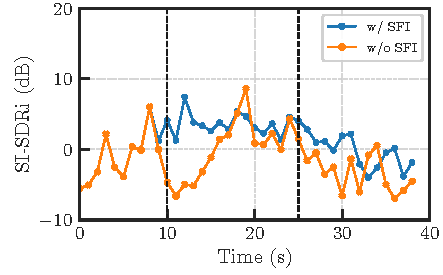
\includegraphics[scale=\myscale]{figures/plots/online/Gauss_8000_97.pdf}
    \caption{$\SubFreq = 8000$}
  \end{subfigure}
  \caption{Frame-wise SI-SDR improvements (dB) with varying $\SubFreq$ where $\forget = 0.97$.}
  \label{fig:online:97}
\end{figure*}
\begin{figure*}[h]
  \centering
  \begin{subfigure}[t]{.3\textwidth}
    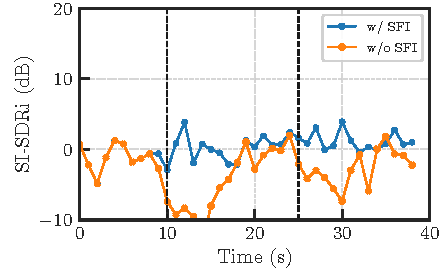
\includegraphics[scale=\myscale]{figures/plots/online/Gauss_2000_99.pdf}
    \caption{$\SubFreq = 2000$}
  \end{subfigure}
  \begin{subfigure}[t]{.3\textwidth}
    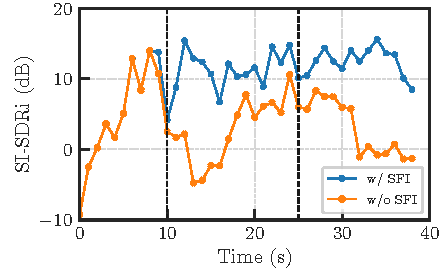
\includegraphics[scale=\myscale]{figures/plots/online/Gauss_4000_99.pdf}
    \caption{$\SubFreq = 4000$}
  \end{subfigure}
  \begin{subfigure}[t]{.3\textwidth}
    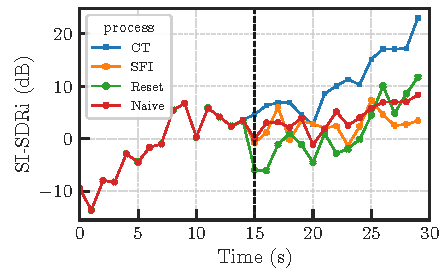
\includegraphics[scale=\myscale]{figures/plots/online/Gauss_8000_99.pdf}
    \caption{$\SubFreq = 8000$}
  \end{subfigure}
  \caption{Frame-wise SI-SDR improvements (dB) with varying $\SubFreq$ where $\forget = 0.99$.}
  \label{fig:online:99}
\end{figure*}
\begin{figure*}[h]
  \centering
  \begin{subfigure}[t]{.3\textwidth}
    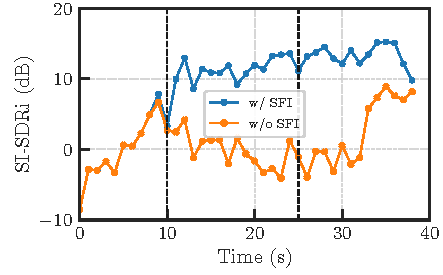
\includegraphics[scale=\myscale]{figures/plots/online/Gauss_2000_995.pdf}
    \caption{$\SubFreq = 2000$}
  \end{subfigure}
  \begin{subfigure}[t]{.3\textwidth}
    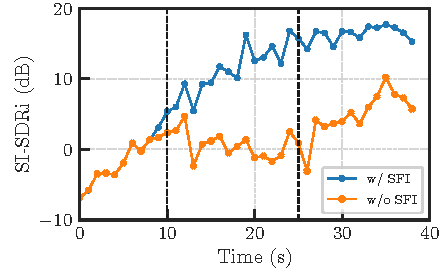
\includegraphics[scale=\myscale]{figures/plots/online/Gauss_4000_995.pdf}
    \caption{$\SubFreq = 4000$}
  \end{subfigure}
  \begin{subfigure}[t]{.3\textwidth}
    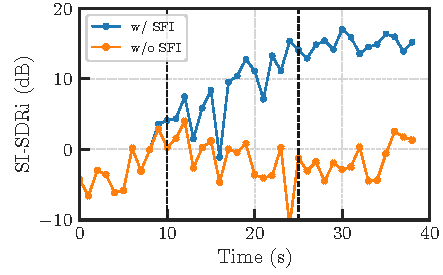
\includegraphics[scale=\myscale]{figures/plots/online/Gauss_8000_995.pdf}
    \caption{$\SubFreq = 8000$}
  \end{subfigure}
  \caption{Frame-wise SI-SDR improvements (dB) with varying $\SubFreq$ where $\forget = 0.995$.}
  \label{fig:online:995}
\end{figure*}

\end{document}
